\section{Introduction}
\label{sec:intro}

Pathology foundation models adapted with LoRA are among the strongest classifiers of mitotic figures on unseen domains
\citep{ammeling2026benchmarking}, but the four we use have 0.3 to 1.2
billion parameters and classify 80 to 342 cells per second on a workstation GPU, 68 to 287 times fewer than a
ResNet-18. Because a whole slide holds thousands of mitosis candidates, the natural route to deployment is to distil the
foundation model into a small task-specific network \citep{hinton2015distilling} that commits to one decision threshold.

Whether the teacher's scanner robustness survives this step is not known. Distilled pathology encoders keep most of
their teachers' average downstream performance, and one was reported to be more robust to scanner variation than its
teacher in embedding space \citep{filiot2025distilling,cai2026deployment,lenz2026multi}. These evaluations,
however, use threshold-free measures. Under scanner shift, the probabilities of foundation models drift even when their
AUC does not \citep{thiringer2026scanner,wen2026tempering}, so a threshold chosen on source scanners can fail on a new
scanner without any loss in ranking \citep{roschewitz2023automatic}. Embedding similarity and AUC hide this failure;
F1 at the deployed operating point exposes it. No study has measured, at that operating point, how much of a foundation
model's scanner robustness a small distilled student keeps, where the rest goes, and what it costs to get it back.

We do so for cell-level mitotic-figure classification on the breast subset of MIDOG++, holding out
one scanner at a time. We distil four LoRA-adapted foundation models into ResNet-18 and ConvNeXt-T students, describe the student's loss on the unseen scanner in three layers, the
\emph{operating point}, the \emph{normalisation statistics} and the \emph{representation}, and repair them in order of
cost (\figureref{fig:schematic}). We ask:
\textbf{RQ1} Does distillation carry the teacher's scanner robustness to the student?
\textbf{RQ2} Where does the student--teacher gap sit?
\textbf{RQ3} What does each layer need to be repaired, and what is the teacher needed for?
\textbf{RQ4} How close does the repaired student get to its teacher, and at what cost?
To separate the teacher's contribution from that of the unlabelled target images, we include controls without any
foundation model; to guard against selective reporting, every confirmatory contrast was specified before the
corresponding models were trained.

\begin{figure}[t]
\floatconts
  {fig:schematic}
  {\caption{Study design. On an unseen scanner, the distilled student's loss is described in three layers, each repaired
  by a step that needs more than the previous one.}}
  {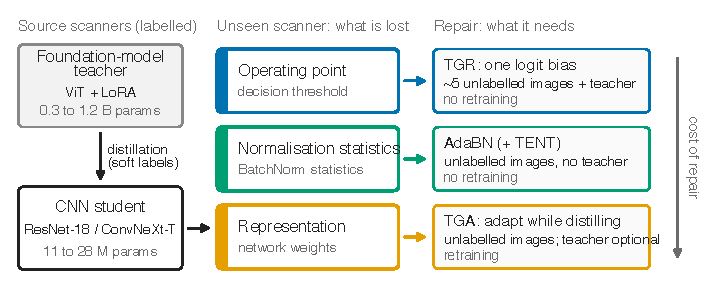
\includegraphics[width=0.9\linewidth]{figures/fig1_schematic}}
\end{figure}

We find: \textbf{(1) Distillation transfers ranking, not robustness.} No teacher gives the ResNet-18 student a
significant F1 gain on the unseen scanner, although its AUROC improves; the ConvNeXt-T student recovers 36\% to 63\% of
the teacher's advantage.
\textbf{(2) The gap is layered, and the layers depend on the student.} For ResNet-18, the operating point and
the BatchNorm statistics account for 51\% to 75\% of the teacher's advantage with three of the four teachers and are
repaired without retraining; for the BatchNorm-free ConvNeXt-T, the operating point alone accounts for 41\% to 46\%.
\textbf{(3) The teacher matters most at the operating point, where it supplies the target prevalence.} One logit
offset fitted to the teacher's predictions on unlabelled images (TGR) reaches the labelled-cutoff bound, to within
0.005 F1 from five images on, and, unlike source-referenced recalibration and prior-shift estimators, survives a change
in prevalence. Most of the retraining gain comes from the unlabelled images rather than from the teacher (75\% to 96\%
for ResNet-18, 57\% for ConvNeXt-T), though for ConvNeXt-T the teacher still adds 0.030 F1.
\textbf{(4) A repaired small student comes close to its teacher.} A ConvNeXt-T student with 23 to 41 times
fewer parameters and 62 to 98 times the throughput recovers 86\% to 99\% of its teacher's advantage and is non-inferior
to Virchow2 at a margin of 0.02 F1; against three LoRA trainings of H-optimus-0 it trails by 0.005 to 0.012 F1, and
non-inferiority is not established. This is an analysis study: TGR is an intercept-only recalibration whose new element is its reference. The contribution
is the measured decomposition, the controls that attribute each repair to the teacher or to the target data, and the
cost-ordered guidance they give for deploying distilled models on new scanners.
